\chapter{RESULT}\label{ch:result}

\section{Demonstration Setup}\label{sec:demonstration}
The results in this chapter are based on the demonstrated Android prototype. The available
evidence consists of application screenshots in indoor settings, showing everyday objects and
groups of people. The screenshots display a confidence threshold of 0.25 and an IoU threshold of
0.70, together with task controls and runtime readings.

These exhibits document the prototype's visible behavior. The available material does not identify
the device model, annotated test-set size, model input resolution, execution backend, or timing
sample duration. Consequently, the reported values are transcriptions of displayed readings, and
the visual demonstrations are not presented as a controlled accuracy benchmark.

\label{end:demonstration}
\section{Visual Output}\label{sec:visual}

\subsection{Detection, Segmentation, and Pose Modes}
Figure~\ref{fig:result-modes} presents three portrait demonstrations. The detection exhibit labels
scissors with a displayed score of 94.2. The segmentation exhibit shows colored regions and labels
for ordinary indoor objects. The pose exhibit combines person boxes with connected body keypoints
in a group scene. Together, these outputs demonstrate that the application can present distinct
computer-vision tasks through the same camera interface.

\begin{figure}[htbp]
  \centering
  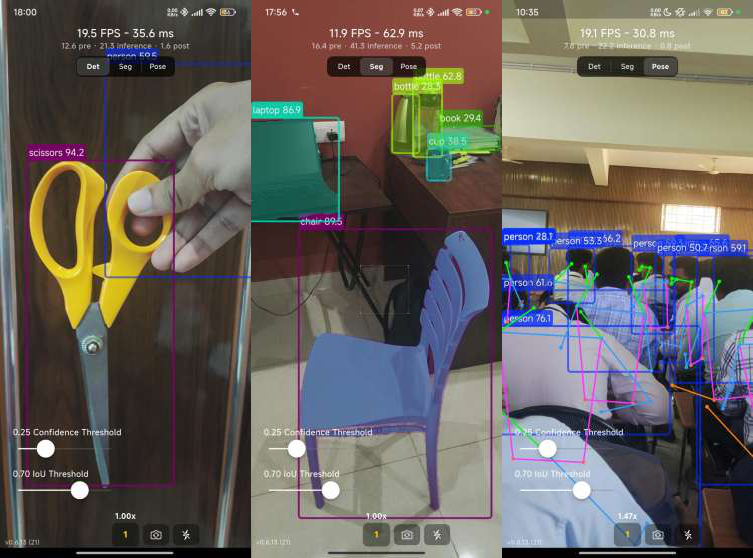
\includegraphics[width=\textwidth]{images/result-modes.png}
  \caption[Detection, Segmentation, and Pose]{Detection, segmentation, and pose outputs from the
    demonstrated prototype.}
  \label{fig:result-modes}
\end{figure}

\subsection{Landscape Object Detection}
The tabletop exhibit in Figure~\ref{fig:result-tabletop} displays a mouse and scissors with scores
of 95.2 and 92.9 respectively. The boxes correspond to the visible objects in the landscape view.
These values are model confidence scores for the displayed predictions; they are not percentages
of correct detections over a test dataset.

\begin{figure}[htbp]
  \centering
  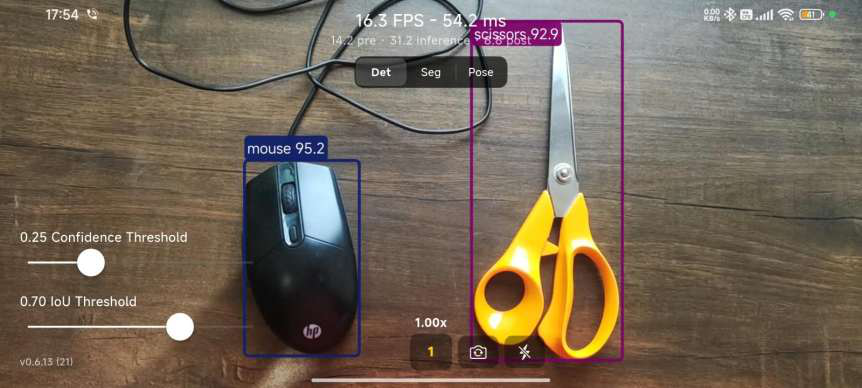
\includegraphics[width=\textwidth]{images/result-tabletop.png}
  \caption[Landscape Object Detection]{Landscape object-detection output from the demonstrated
    prototype.}
  \label{fig:result-tabletop}
\end{figure}

\subsection{Segmentation and Group Pose Visualization}
Figure~\ref{fig:result-interior} shows the interior scene. The screenshot includes region overlays
and labels for a couch, vase, laptop, and bottle. The displayed bottle score is 28.6, which is
above the configured 25\% confidence threshold but substantially lower than the laptop score of
90.3. This illustrates why per-object confidence and visual checking matter when interpreting the
output.

\begin{figure}[htbp]
  \centering
  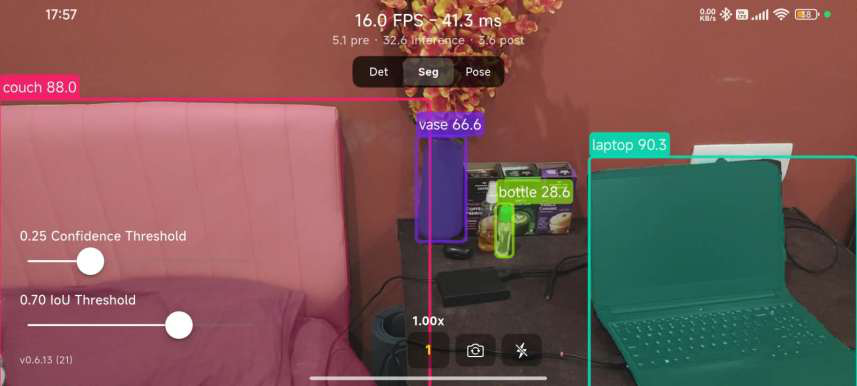
\includegraphics[width=\textwidth]{images/result-interior.png}
  \caption[Indoor Segmentation Output]{Indoor segmentation output from the demonstrated prototype.}
  \label{fig:result-interior}
\end{figure}

The group scene in Figure~\ref{fig:result-pose} contains multiple person boxes and connected pose
keypoints, including partially occluded subjects. This establishes that multi-person overlays were
displayed in the demonstrated scene. It does not quantify pose accuracy, tracking consistency, or
performance under battlefield conditions.

\begin{figure}[htbp]
  \centering
  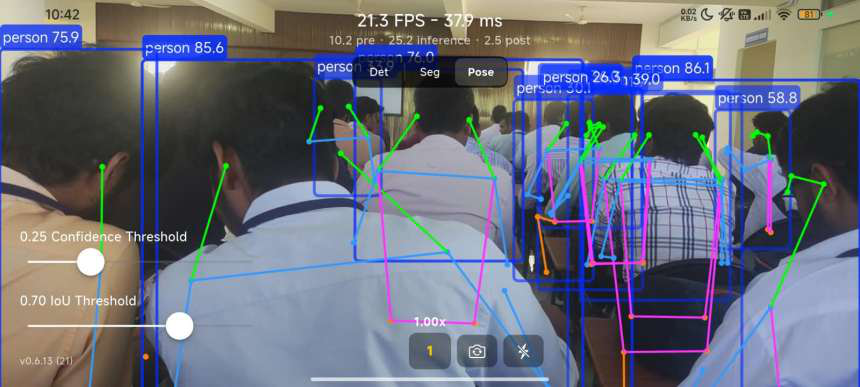
\includegraphics[width=\textwidth]{images/result-pose.png}
  \caption[Multi-Person Pose Output]{Multi-person pose output from the demonstrated prototype.}
  \label{fig:result-pose}\label{end:visual}
\end{figure}

% Finish the visual evidence before discussing the numerical readings.
\clearpage
\section{Displayed Runtime Measurements}\label{sec:runtime}
Table~\ref{tab:runtime} records the frame-rate and processing-time readings visible in the six
exhibits. The values span 11.9--21.3 FPS and 30.8--62.9 ms of displayed processing time. They
refer to different scenes and task modes, so they should not be treated as an average over one
uniform experiment or used to rank model variants without additional test controls.

\begin{table}[htbp]
  \centering
  \caption{Displayed Runtime Readings}\label{tab:runtime}
  \begin{tabular}{p{7.3cm}crr}
    \toprule
    \textbf{Exhibit} & \textbf{View} & \textbf{FPS} & \textbf{Time (ms)} \\
    \midrule
    Exhibit A: Portrait scissors detection & Portrait & 19.5 & 35.6 \\
    Exhibit B: Portrait segmentation & Portrait & 11.9 & 62.9 \\
    Exhibit C: Portrait group pose & Portrait & 19.1 & 30.8 \\
    Exhibit D: Landscape mouse and scissors & Landscape & 16.3 & 54.2 \\
    Exhibit E: Landscape interior segmentation & Landscape & 16.0 & 41.3 \\
    Exhibit F: Landscape group pose & Landscape & 21.3 & 37.9 \\
    \bottomrule
  \end{tabular}
\end{table}

The landscape segmentation screenshot decomposes its 41.3 ms reading into 5.1 ms preprocessing,
32.6 ms inference, and 3.6 ms post-processing. The group-pose screenshot similarly shows 10.2 ms,
25.2 ms, and 2.5 ms, totaling 37.9 ms. In both snapshots, inference is the largest displayed
component, making model execution an important target for further profiling.

The displayed FPS is not simply the reciprocal of the processing-time field. For instance, 37.9 ms
corresponds to approximately 26.4 processing cycles per second, whereas the screenshot reports
21.3 FPS. Capture, scheduling, rendering, and the application's averaging conventions can affect
the relationship between these indicators. The timing windows are not defined, so the
processing-time field is not claimed to measure end-to-end camera-to-display latency.

\label{end:runtime}
\section{Discussion and Limitations}\label{sec:discussion}
The demonstration shows a functional foundation: live camera input, on-device inference,
task-specific visualization, configurable thresholds, and displayed runtime information. The
exhibits support continued development of a portable situational-awareness application. They also
show that the demonstrated classes are predominantly ordinary objects and people, rather than a
validated combat-specific threat vocabulary.

Quantitative accuracy evaluation requires an annotated dataset and a defined test split. Precision,
recall, and mAP are not reported for the current prototype because the available material does not
contain the necessary measurements. Similarly, sustained FPS, latency distributions, power
consumption, and thermal behavior require repeated runs on a documented device. Numerical results
reported for papers in the literature review remain results of those studies, not measurements of
VeerDrishti.

Further evaluation should cover small or distant objects, occlusion, camera motion, illumination
changes, false detections, missed detections, and overlay alignment. Combat-specific fine-tuning,
thermal fusion, open-vocabulary recognition, and persistent event storage should be documented
with their own implementation and evaluation evidence when completed. The current results
therefore establish demonstrated prototype behavior while leaving robustness and operational
effectiveness to be assessed through controlled testing.
\label{end:discussion}\label{end:result}
